\documentclass[11pt,a4paper]{article}
\usepackage[utf8]{inputenc}
\usepackage[T1]{fontenc}
\usepackage[margin=2.5cm]{geometry}
\usepackage{graphicx}
\usepackage{booktabs}
\usepackage{array}
\usepackage{float}
\usepackage{enumitem}
\setlist{nosep}
\usepackage{tikz}
\usetikzlibrary{positioning,arrows.meta,fit,backgrounds}
\usepackage{hyperref}

\title{TrialMatch: report}
\author{Yuliia Lytvynenko}
\date{\today}

\begin{document}
\maketitle

\begin{center}
\textbf{Code:} \href{https://github.com/juliatvenko/ucu-gen-ai-nlp-system}{github.com/juliatvenko/ucu-gen-ai-nlp-system}\\[4pt]
\textbf{Video recording with the defense:} \href{https://drive.google.com/drive/folders/1kLgAYUDZJBdlDy1W_TkI722TyYLyGJNW}{Google Drive folder}\\
\small (opens only when signed in with a UCU email account)
\end{center}

% Brief: "Define the Task".
\section{Task and scope}

Finding a clinical trial means reading the eligibility criteria of many trials and comparing each with the patient. This takes a lot of time. TrialMatch helps clinicians and trial coordinators do it. For each criterion it returns \emph{met}, \emph{not met} or \emph{insufficient data}, with a quote from the patient text as evidence. Plain code turns these into a verdict, and the system asks for the missing facts that matter most.

It has two modes on one engine. \textbf{Matcher:} one patient, ranked trials. \textbf{Cohort:} one trial, a set of patients, who could qualify. The system is more than RAG: retrieval only finds candidates, and the core is extraction, a decision per criterion with a required quote, and rule-based verdicts.

\textbf{Success} means catching patients who fail a criterion, showing the reason for every decision, and saying ``insufficient data'' when the text does not settle a criterion. \textbf{The most costly errors}, in order: a status without evidence, an excluded patient shown as eligible, and an eligible trial not shown.

\textbf{In scope:} age and sex filters; a status for every criterion; verdicts by code; follow-up questions; cohort search over 1,620 case reports; stopping on urgent, off-topic and advice-only input; a labelled rule fallback in the app. \textbf{Out of scope:} trial location, hosted deployment, real patient data.

\textbf{Ethics.} The tool is assistive: it quotes its basis, and clinicians make the final decision. Unmentioned facts count as missing, not as evidence. Only synthetic and published data are used, because free model endpoints may train on their inputs.

\textbf{Related work.} Checking each criterion separately follows TrialGPT (Jin et al., 2024). No code was reused. TrialMatch adds two modes on one engine, a parsing eval on Chia, and a safety metric for how often the system says ``insufficient data'' when it should.

% Brief: "Prepare the Data (check existing datasets before generating synthetic)".
\section{Data}

I checked existing datasets first. Real, human-labelled data is used where it exists, and synthetic data only fills gaps.

\begin{table}[!htb]
\centering
\small
\begin{tabular}{>{\raggedright\arraybackslash}p{3.3cm}>{\raggedright\arraybackslash}p{3.4cm}>{\raggedright\arraybackslash}p{3.6cm}>{\raggedright\arraybackslash}p{3.3cm}}
\toprule
Dataset & Size & Used for & Labels \\
\midrule
Chia (CC BY 4.0) & 1,000 trials & Parsing eval, list of medical phrases & Human entity annotations \\
TREC Clinical Trials 2021 & 75 patients, 35,832 judgements & Retrieval, cohort search, end-to-end evals & Human: not relevant, excluded, eligible \\
ClinicalTrials.gov API v2 & Live registry & Trials in the app & None \\
PMC-Patients (CC BY-NC-SA 4.0) & 1,620 case reports & Demo examples, cohort search & None, so not in evals \\
\texttt{vignettes.json} & 16 patients, 128 pairs & Profile and checker evals & Synthetic \\
\texttt{safety\_cases.json} & 24 inputs & Safety eval & Synthetic \\
\texttt{parsing\_gold.json} & 10 texts & Segmentation eval & Synthetic \\
\bottomrule
\end{tabular}
\caption{Datasets and their use.}
\end{table}

TREC is the main end-to-end test, because its labels come from people. n2c2 2018 was rejected because it needs a data use agreement. The coding agent wrote the synthetic sets, and I reviewed the vignette labels. The safety cases were used to fix the rules, so they only check that fixed cases stay fixed (a regression test), not how the rules handle new input.

\textbf{Splits.} Chia by trial (800/100/100), TREC by topic (1--37 dev, 38--75 test, 2 trials per label in model runs), vignettes by patient (8/8). Dev is for tuning and test is for reporting: I tuned on dev only and did not read test errors. All preparation is scripted, and raw data is never edited.

% Brief: "Describe the Components". Criterion: System understanding, 7 pts.
\section{System}

Both modes use the same engine (Figure~\ref{fig:flow}). They differ only in where the patient and trial come from.

\begin{figure}[H]
\centering
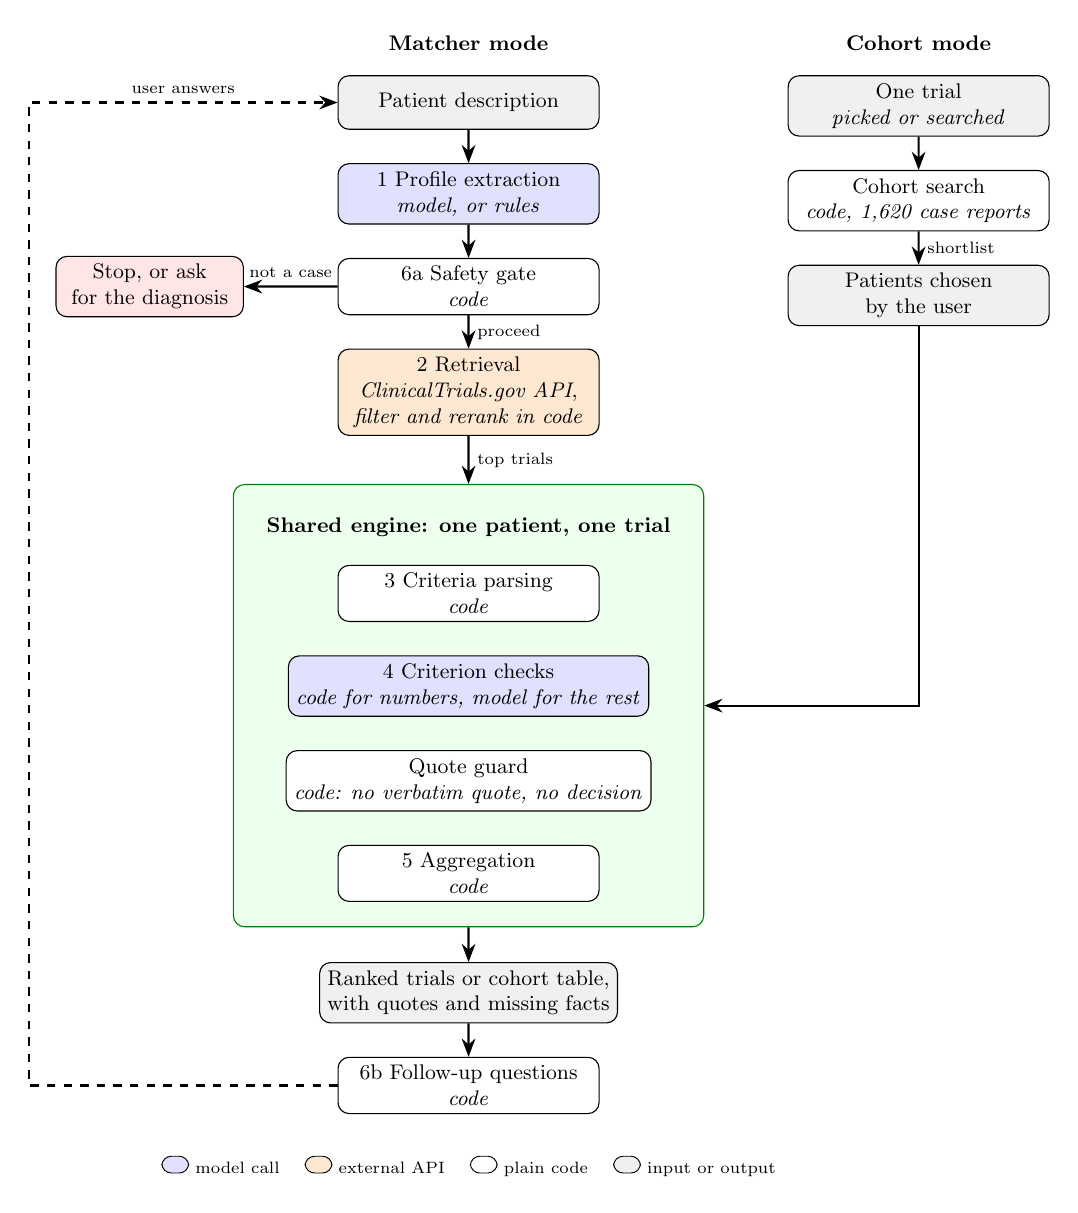
\begin{tikzpicture}[scale=0.85, every node/.style={transform shape},
  node distance=0.5cm and 0.6cm,
  box/.style={draw, rounded corners, align=center, font=\small, minimum width=3.9cm, minimum height=0.8cm},
  io/.style={box, fill=gray!12},
  model/.style={box, fill=blue!12},
  code/.style={box, fill=white},
  tool/.style={box, fill=orange!18},
  stop/.style={box, fill=red!10, minimum width=2.8cm},
  arr/.style={-{Stealth}, thick},
  lab/.style={font=\scriptsize},
  head/.style={font=\small\bfseries}
]
% Matcher mode
\node[head] (mh) {Matcher mode};
\node[io, below=0.25cm of mh] (in) {Patient description};
\node[model, below=of in] (prof) {1 Profile extraction\\\textit{model, or rules}};
\node[code, below=of prof] (safe) {6a Safety gate\\\textit{code}};
\node[stop, left=1.4cm of safe] (stop) {Stop, or ask\\for the diagnosis};
\node[tool, below=of safe] (ret) {2 Retrieval\\\textit{ClinicalTrials.gov API},\\\textit{filter and rerank in code}};

% Cohort mode
\node[head, right=4.2cm of mh] (ch) {Cohort mode};
\node[io, below=0.25cm of ch] (trial) {One trial\\\textit{picked or searched}};
\node[code, below=of trial] (cs) {Cohort search\\\textit{code, 1,620 case reports}};
\node[io, below=of cs] (pts) {Patients chosen\\by the user};

% Shared engine
\node[head, below=1.1cm of ret] (etitle) {Shared engine: one patient, one trial};
\node[code, below=0.3cm of etitle] (parse) {3 Criteria parsing\\\textit{code}};
\node[model, below=of parse] (check) {4 Criterion checks\\\textit{code for numbers, model for the rest}};
\node[code, below=of check] (guard) {Quote guard\\\textit{code: no verbatim quote, no decision}};
\node[code, below=of guard] (agg) {5 Aggregation\\\textit{code}};
\begin{scope}[on background layer]
  \node[draw=green!50!black, fill=green!7, rounded corners, inner sep=9pt, fit=(etitle)(parse)(check)(guard)(agg)] (eng) {};
\end{scope}

\node[io, below=0.9cm of agg] (out) {Ranked trials or cohort table,\\with quotes and missing facts};
\node[code, below=of out] (fu) {6b Follow-up questions\\\textit{code}};

% Arrows
\draw[arr] (in) -- (prof);
\draw[arr] (prof) -- (safe);
\draw[arr] (safe) -- node[lab, above]{not a case} (stop);
\draw[arr] (safe) -- node[lab, right]{proceed} (ret);
\draw[arr] (ret) -- node[lab, right]{top trials} (eng.north -| ret);
\draw[arr] (trial) -- (cs);
\draw[arr] (cs) -- node[lab, right]{shortlist} (pts);
\draw[arr] (pts) |- (eng.east);
\draw[arr] (eng.south -| agg) -- (out);
\draw[arr] (out) -- (fu);
\draw[arr, dashed] (fu.west) -- ([xshift=-0.4cm]fu.west -| stop.west) |- node[lab, above, pos=0.75]{user answers} (in.west);

% Legend
\node[below=0.5cm of fu, font=\scriptsize, align=center] {
  \tikz\node[draw, rounded corners, fill=blue!12, minimum width=0.4cm, minimum height=0.25cm]{}; model call \quad
  \tikz\node[draw, rounded corners, fill=orange!18, minimum width=0.4cm, minimum height=0.25cm]{}; external API \quad
  \tikz\node[draw, rounded corners, fill=white, minimum width=0.4cm, minimum height=0.25cm]{}; plain code \quad
  \tikz\node[draw, rounded corners, fill=gray!12, minimum width=0.4cm, minimum height=0.25cm]{}; input or output};
\end{tikzpicture}
\caption{Data flow in both modes.}
\label{fig:flow}
\end{figure}

\begin{table}[!htb]
\centering
\small
\begin{tabular}{>{\raggedright\arraybackslash}p{2.5cm}>{\raggedright\arraybackslash}p{5.2cm}>{\raggedright\arraybackslash}p{3.2cm}>{\raggedright\arraybackslash}p{3.2cm}}
\toprule
Component & Purpose & Input & Output \\
\midrule
1 Profile & Turn free text into structured facts & Patient text & Age, sex, diagnoses, labs, drugs \\
2 Retrieval & Find candidate trials, drop impossible ones & Profile & Ranked trials \\
3 Parsing & Split eligibility text into criteria, keep its structure & Eligibility text & Criteria \\
4 Checker & Decide each criterion, with a quote & Criteria, patient text & Status, quote, reason \\
5 Aggregation & Turn statuses into a verdict & Criteria, checks & Verdict \\
6a Safety & Decide whether to run at all & Text, profile & Proceed, stop or ask \\
6b Follow-up & Ask for the most useful missing facts & Verdicts & Questions \\
\bottomrule
\end{tabular}
\caption{Components.}
\end{table}

A trial is \textbf{not eligible} if an inclusion is not met or an exclusion is met. Otherwise it is \textbf{likely eligible}, \textbf{needs more data} or \textbf{insufficient data}, by how many criteria are unknown. Parsing keeps the trial's structure: a list of options (``one of the following'') counts as one criterion, a criterion for one group only (``for women of child-bearing potential'') cannot block alone, and sections about a donor or relative are skipped. Cohort search ranks case reports by keyword match (BM25), with no model.

\textbf{Model calls.} The model is \texttt{gemini-3.5-flash-lite} (Google AI Studio, free tier), used in two places. Everything else is code. The only external tool is the ClinicalTrials.gov API v2.

\begin{table}[!htb]
\centering
\small
\begin{tabular}{>{\raggedright\arraybackslash}p{1.6cm}>{\raggedright\arraybackslash}p{2.4cm}>{\raggedright\arraybackslash}p{2.9cm}>{\raggedright\arraybackslash}p{3.6cm}>{\raggedright\arraybackslash}p{3.3cm}}
\toprule
Step & Model gets & Model returns & Code then & Why a model \\
\midrule
1 Profile & Patient text & JSON: age, sex, diagnoses, drugs, labs, history, absent facts & Safety gate checks it; retrieval uses the diagnosis, age and sex & Abbreviations, drug names, negation (``denies \ldots'') \\
4 Checker & Patient text, up to 40 criteria per call & Status, quote and reason per criterion & Drops decisions without a verbatim quote, applies inclusion or exclusion, makes the verdict & Drug classes, synonyms, loosely worded criteria \\
\bottomrule
\end{tabular}
\caption{Where the model is used.}
\end{table}

Consent criteria and simple numbers never reach the model, and it never decides eligibility. All calls go through \texttt{llm.py}, which validates JSON, caches answers and logs a trace. Each model step has a rule version, used as the baseline and the fallback.

\textbf{Why this design.} The model judges language; code decides, checks and counts. Inclusion versus exclusion, numbers and the verdict stay in code, so they are predictable and auditable. The quote guard is code, because a prompt cannot prove a quote is real. \emph{Insufficient} lets the system say ``not enough information'' and drives the follow-up questions.

\textbf{One input through the system} (vignette \texttt{d01}, \texttt{scripts/trace\_input.py}):
\begin{enumerate}
  \item \textbf{Input:} ``58-year-old woman with type 2 diabetes\ldots{} HbA1c 8.4\%\ldots{} She denies any history of heart failure.''
  \item \textbf{Profile:} age 58, female, \emph{type 2 diabetes}, \emph{HbA1c = 8.4}, absent \emph{heart failure}.
  \item \textbf{Safety:} a diagnosis, nothing urgent, so proceed.
  \item \textbf{Retrieval:} recruiting trials for ``type 2 diabetes'', filtered by age and sex, top 5 after ranking by keyword match.
  \item \textbf{Parsing:} criteria per trial; ``Signed informed consent'' is left to study staff.
  \item \textbf{Checks:} ``HbA1c 7.0--9.0\%'' is \emph{met} in code. ``History of heart failure'' is \emph{not met}, quote ``denies any history of heart failure''. ``Myocardial infarction within 6 months'' is \emph{insufficient}.
  \item \textbf{Aggregation:} no blockers, some unknown: \emph{needs more data}.
  \item \textbf{Follow-up:} ``Has the patient had myocardial infarction?'' The answer is added, and the steps run again.
\end{enumerate}

\textbf{Interface.} A FastAPI server streams results to a React app, which shows each status with its quote highlighted in the patient text. Rule fallback results are labelled ``Rules only''.

% Brief: "Evaluate the System". Criterion: Evaluation, 7 pts.
\section{Evaluation}

Each component has an eval in \texttt{evals/}, run with rules (baseline) and with the model. Numbers come from \texttt{evals/results/}, test split.

\begin{table}[!htb]
\centering
\footnotesize
\begin{tabular}{>{\raggedright\arraybackslash}p{1.9cm}>{\raggedright\arraybackslash}p{4.8cm}>{\raggedright\arraybackslash}p{2.6cm}>{\raggedright\arraybackslash}p{2.2cm}>{\raggedright\arraybackslash}p{2.2cm}}
\toprule
Component & Metric & Data & Rules & Model \\
\midrule
1 Profile & F1: diagnoses / medications / absent facts & Vignettes & .86 / .35 / .57 & .91 / .96 / 1.0 \\
2 Retrieval & Search query recall / precision & TREC 2021 & .27 / .47 & .47 / .77 \\
 & Ranking quality, nDCG@10 (random .48) & TREC 2021 & .51 & .63 \\
 & Trials outside age/sex limits & Vignettes, live & 0 & 0 \\
2b Cohort search & Eligible patient in top 10 (random .14) & TREC, reversed & .92 & -- \\
3 Parsing & Splitting into criteria F1, bulleted / plain & Chia & 1.0 / .87 & same \\
 & Entity F1, exact / overlapping span & Chia & .36 / .55 & .47 / .74 \\
4 Checker & Macro-F1 (n=64) & Vignettes & .61 & .90 \\
 & Quotes verbatim / flip rate & Vignettes & 1.0 / .04 & 1.0 / 0 \\
 & Decided where gold is \emph{insufficient} & Vignettes & .07 & .27 \\
5 Aggregation & All status combinations / missed blocks & All combinations / vignettes & 100\% / .2 & 100\% / 0 \\
6a Safety & Macro-F1, authored cases & \texttt{safety\_cases} & 1.0 & 1.0 \\
6b Follow-up & Settled correctly after an answer & Vignettes & 0 & 1.0 \\
\midrule
End to end & Eligible vs excluded F1 (n=76) & TREC 2021 & .70 & .72 \\
 & Excluded trials caught (95\% CI) & TREC 2021 & .19 [.12, .29] & .67 [.55, .76] \\
\bottomrule
\end{tabular}
\caption{Results per component, test split. Full results for both splits: \texttt{evals/results/}.}
\end{table}

\textbf{Why these metrics.} Classes are imbalanced, so I use per-class precision, recall and macro-F1, not accuracy. The checker has two safety metrics: unsupported decisions (the text does not mention the fact, but the checker still says \emph{met} or \emph{not met} instead of \emph{insufficient}) and the flip rate (\emph{met} read as \emph{not met}). Search query recall and precision count the human-judged trials the query finds. nDCG@10 scores the order of the top 10. End to end is compared with a baseline that never marks a trial \emph{not eligible}.

\textbf{Reading the results.} The model helps most where language varies: drug classes, abbreviations, negation, and follow-up answers. End-to-end F1 is similar (.70 and .72), but the errors are opposite: the rules rarely block, and the model catches more excluded trials but also blocks some eligible ones. The main remaining issue is unsupported decisions: on 27\% of criteria the text does not mention, the model still answers \emph{met} or \emph{not met}. It quotes real text that is not about the criterion, so the quote guard can't catch it.

\textbf{Error analysis.} I read all 39 dev errors. Of 25 eligible trials marked \emph{not eligible}, 11 came from parsing losing the trial's structure, 12 from TREC labels that say ``eligible'' when the trial text excludes the patient, and 2 from the model reading more into the text than it says. I fixed the parsing group: dev F1 .715 $\to$ .761, test .705 $\to$ .722, with no new errors.

\textbf{Trust.} Verbatim quotes, the status combinations and the age/sex limits are correct by design: the code enforces them. Vignette scores are likely higher than on real text, because the texts are short and clear. Safety 1.0 is a regression test. TREC is the most credible test, but small.

% Brief: "it should be reflected in your report how you applied it".
\section{CRISP-DM}

\texttt{AGENTS.md} lists what the agent must do in each phase. The agent states the phase before a change and records decisions in \texttt{docs/crisp\_dm.md}, using the \texttt{crisp-dm-checkpoint} skill.

\begin{table}[!htb]
\centering
\small
\begin{tabular}{>{\raggedright\arraybackslash}p{2.6cm}>{\raggedright\arraybackslash}p{11.6cm}}
\toprule
Phase & What I did and decided \\
\midrule
Business & Users, success criteria, costly errors in order, scope. \\
Data understanding & Counted and sampled each dataset before coding. Rejected n2c2; added TREC for its human labels. \\
Data preparation & Scripts only; splits by trial, topic and patient; synthetic data only for gaps. \\
Modeling & Code parts first, then the model for profile and checker. Rules kept as the baseline. \\
Evaluation & An eval per component, before and after each change. Dev only; prompts frozen before the test run. \\
Deployment & Local FastAPI and React app, checked in a browser. Rule fallback in the app only. \\
\bottomrule
\end{tabular}
\caption{CRISP-DM phases.}
\end{table}

\textbf{Going back a phase} happened six times:
\begin{itemize}
  \item \textbf{Evaluation $\to$ Data preparation:} low Chia scores showed that line-ending conversion shifted text positions; files are now read without conversion.
  \item \textbf{Deployment $\to$ Modeling:} live trials showed rule bugs, for example only one bound checked in ``Age $\geq$ 21 and $\leq$ 65''.
  \item \textbf{Evaluation $\to$ Modeling:} the model decided on 44\% of unmentioned dev criteria; a stricter prompt lowered this to 19\%.
  \item \textbf{Evaluation $\to$ Modeling:} ``no known allergies'' was read as a diagnosis; the rules now check negation.
  \item \textbf{Evaluation $\to$ Modeling:} the dev error analysis led to the parsing structure fix.
  \item \textbf{Deployment $\to$ Modeling:} retrieval searched for ``the right leg''; it no longer searches for a body part alone.
\end{itemize}

\section{Limitations}

Small gold sets, so intervals are wide. One free model, which may change. Unsupported decisions on facts the text does not mention. Statuses can change after a small edit to the patient text (not measured). TREC labels are from 2021, but trial text is current. Prompt injection is not measured. Cohort search was tuned on TREC notes, not on the case reports it searches. No location logic.

% Criterion: Use of the AI coding assistant, 4 pts.
\section{AI coding assistant}

I built the system with Claude Code and steered it with files, not only prompts.

\textbf{AGENTS.md} (62 lines; \texttt{CLAUDE.md} only imports it) has five parts: the CRISP-DM process; eval integrity (dev only, no hand-written metrics, never change a gold label); system rules (the model never decides, decisions need a verbatim quote, an unmentioned fact is not evidence, evals never switch to rules when the model fails); project limits (no work data, no private data, no copied code); and code conventions with the test command.

\textbf{Skills:} \texttt{run-evals} (before and after scores), \texttt{crisp-dm-checkpoint} (log a phase decision), \texttt{trace-input} (one input through every component).

\textbf{Context.} \texttt{AGENTS.md} loads in every session, skills only when needed. Long sessions lose context, so decisions, errors and scores are written to files (\texttt{crisp\_dm.md}, \texttt{error\_analysis\_dev.md}, \texttt{evals/results/}), and a new session reads them.

\subsection*{Reflection}

\textbf{What I left out of context.} My work data and code (NDA), even though my job is close to this topic. Private and restricted data: I dropped n2c2 and used open data only. Other people's code: the agent got the idea of TrialGPT, not its repositories. Also the API keys and the test errors.

\textbf{What worked.} The eval rules mattered most: ``dev only'' kept the test score independent of tuning, and ``a decision needs a verbatim quote'' made answers checkable. Real runs found bugs that tests missed.

\textbf{Corrections I made.} Many, mostly in the interface. The agent also did not start improvement cycles by itself, so I led the error analysis and fixes.
\begin{itemize}
  \item Streamlit replaced by FastAPI and React.
  \item A better error message replaced by a labelled rule fallback.
  \item AI-generated demo patients replaced by published case reports.
  \item A trial picker added, and a case report search built only after its eval.
  \item Gold labels reviewed; only the parsing errors fixed; claims in this report made more precise.
\end{itemize}

\textbf{Problems.} The agent once reported results as saved before saving them, and the test command in \texttt{AGENTS.md} was wrong for most of the project.

\textbf{Next time} I would start \texttt{AGENTS.md} small and add a rule after each repeated mistake, enforce key rules with hooks, add exact commands and examples, and write some test cases myself early.

\section{How to run}

Python 3.11+. Full instructions, including the model key and evals, are in \texttt{README.md}.
\begin{verbatim}
python3 -m venv .venv
.venv/bin/pip install -r requirements.txt
.venv/bin/python -m uvicorn server:app --port 8000   # open localhost:8000
.venv/bin/python -m pytest -q
\end{verbatim}
Without a key, the app runs with the rule baseline. To add the model key, see \texttt{README.md}.

\end{document}
